
%(BEGIN_QUESTION)
% Copyright 2006, Tony R. Kuphaldt, released under the Creative Commons Attribution License (v 1.0)
% This means you may do almost anything with this work of mine, so long as you give me proper credit

It is important for a process chromatograph that the sample injection valve have a continuously flowing source of sample fluid, as well as a continuous exit point for that flowing sample (i.e. a {\it sample supply} and a {\it sample waste} tube leading in and out of the sample injection valve):

$$\includegraphics[width=15.5cm]{i00676x01.eps}$$

If we only provided the sample valve with a single (entry) tube for the sample fluid, the chromatograph's operation would be seriously impaired:

$$\includegraphics[width=15.5cm]{i00676x02.eps}$$

Explain why we need the sample to continuously flow {\it through} the sample valve when it is not injecting sample into the column.

\underbar{file i00676}
%(END_QUESTION)





%(BEGIN_ANSWER)

Process chromatographs only require {\it very} small volumes of sample injected for proper operation.  This is especially true for chromatographs using {\it capillary tubes} for their columns.  Since the volume of injected sample is so incredibly small, a chromatograph with no ``sample out'' flow would take {\it days} to draw a new sample through the volume of the tube connecting the chromatograph to the process pipe.

A continuously flowing sample provides a way for the chromatograph to obtain a ``fresh'' sample at each and every analysis cycle.

%(END_ANSWER)





%(BEGIN_NOTES)


%INDEX% Measurement, analytical: chromatography

%(END_NOTES)


